\documentclass[11pt,letterpaper]{article}

\usepackage[margin=1in]{geometry}
\usepackage[T1]{fontenc}
\usepackage[utf8]{inputenc}
\usepackage{microtype}
\usepackage{amsmath,amssymb}
\usepackage{booktabs}
\usepackage{graphicx}
\usepackage{caption}
\usepackage{authblk}
\usepackage{enumitem}
\usepackage[hyphens]{url}
\usepackage{xcolor}
\usepackage[round,authoryear]{natbib}
\usepackage{hyperref}

\hypersetup{
  pdftitle={High-Beta Acceleration in Low-Debt Tech: An Exploratory Backtest of Upside Participation versus Downside Capture under AAOIFI Screens, 2020-2025},
  pdfauthor={Rao Abdul Hadi},
  pdfsubject={Halal equity investing, high beta, low debt, technology, clean energy, AAOIFI screens},
  pdfkeywords={high beta, downside capture, upside participation, AAOIFI, Sharia-compliant equities, technology, clean energy, backtest},
  colorlinks=true,
  citecolor=blue,
  linkcolor=blue,
  urlcolor=blue
}

\captionsetup{font=small,labelfont=bf,skip=6pt}
\setlength{\parindent}{1.5em}
\setlength{\parskip}{0pt}
\setlist[itemize]{leftmargin=1.5em,itemsep=0.2em,topsep=0.35em}
\setlist[enumerate]{leftmargin=1.5em,itemsep=0.2em,topsep=0.35em}

\renewcommand\Authfont{\normalsize}
\renewcommand\Affilfont{\small}
\setlength{\affilsep}{0.6em}

\title{\textbf{High-Beta Acceleration in Low-Debt Tech:\\
An Exploratory Backtest of Upside Participation versus Downside Capture under AAOIFI Screens, 2020--2025}}

\author[1]{Rao Abdul Hadi\thanks{Corresponding author. Email: \href{mailto:raoabdulhadi952@gmail.com}{raoabdulhadi952@gmail.com}.}}
\affil[1]{Monterey Finance, Halal Quant Research Lab}

\date{September 2026}

\begin{document}
\maketitle

\begin{abstract}
\noindent
This paper asks whether a long-only, high-beta growth book can deliver strong upside participation without corporate leverage risk once Islamic screens are applied. I start from the S\&P~500 plus a liquid clean-energy overlay, keep Technology, Communication Services, and clean-energy names that pass AAOIFI financial-ratio tests (debt below 30\% of market cap, with cash and receivables caps), rank survivors by trailing 252-day OLS beta versus SPY, and own the top quintile in proportion to market cap, rebalanced monthly. From 31~January~2020 through 30~December~2025 the high-beta book returned 34.9\% compound annual growth, against 15.1\% for SPY, 13.4\% for the S\&P~500 index, and 17.7\% for a Halal large-cap ETF (SPUS). An equal-weight Halal tech/clean-energy sleeve---same universe, no beta tilt---returned only 20.3\% CAGR, so the beta sort itself adds about 15~percentage points of annualized return in this sample. The cost is risk: volatility is 43.4\% and maximum drawdown is $-48.8\%$, versus roughly $-31\%$ to $-34\%$ for the benchmarks. Upside capture versus SPY is 1.90 and downside capture is 1.80; the capture spread is only slightly positive. Portfolio beta runs about 1.7--2.2 for most of the sample while weighted debt stays well under 5\%. Beta quintiles inside the sleeve are not monotonic---Q5 leads, but Q3 beats Q1, Q2, and Q4---so the live edge is concentrated in the top bucket rather than a clean ladder. The sample is a growth-friendly window, the book is mega-cap concentrated (Nvidia alone was nearly half the weight at the last rebalance), and there is no sector-neutral twin. The numbers should be read as an exploratory backtest, not as a forecast or a live-return target.
\end{abstract}

\noindent\textbf{Keywords:}
high beta; upside participation; downside capture; AAOIFI; Sharia-compliant equities; technology; clean energy; low debt; backtest.

\noindent\textbf{JEL classification:} G11, G12, Z12.

\noindent\textbf{Code:}
Replication notebook and figures are in the Monterey Finance repository,
\url{https://github.com/regional-specter/Monterey-Finance},
under \path{Research/papers/05-high-beta/}.

\section{Introduction}

Market beta is the simplest description of how hard a stock moves with the broad market. High-beta equities participate more on up days and, typically, lose more on down days \citep{fama1992,black1972}. Growth investors often accept that asymmetry deliberately: they want acceleration in bull markets and hope that security selection, sector focus, or balance-sheet quality will soften the left tail. Corporate leverage is a separate amplifier. Interest-bearing debt raises equity beta for a given asset beta and raises bankruptcy risk in rate or liquidity shocks. Islamic equity screens remove much of that channel before any beta sort is applied. AAOIFI financial-ratio limits cap debt, cash, and receivables relative to market value, and a separate activity screen removes banks, conventional insurance, alcohol, tobacco, gambling, weapons, and similar businesses \citep{aaoifi21,derigs2008}. The economic hope in this paper is therefore specific: \emph{can a top-quintile beta sleeve inside low-debt technology and clean energy deliver growth-like upside without relying on issuer leverage?}

That hope is not automatic. Technology and clean-energy names already dominate Halal large-cap universes after financials are stripped out. A high-beta sort inside that sleeve may simply pick Nvidia, Broadcom, Tesla, and other mega-cap accelerators that already won 2020--2025. Upside participation would then look impressive on CAGR while downside capture remains close to one-for-one with a larger amplitude. The white-paper question is not ``did high beta make money in a bullish sample?'' It is whether the participation asymmetry---upside capture versus downside capture---justifies running an unlevered high-beta growth book under Sharia constraints.

The live rule tested here is narrow. After banned businesses and AAOIFI screens, restrict to Technology, Communication Services, and clean-energy industries, score each name by trailing OLS beta versus SPY, keep the top quintile, and cap-weight monthly. There is no portfolio margin, no short book, and no SMA cash overlay. The comparison set is SPY, the S\&P~500 cash index (\texttt{\^GSPC}), SPUS, and an equal-weight Halal tech/clean-energy twin that isolates the beta tilt from sector membership.

It does deliver headline outperformance. It also takes nearly 50\% peak-to-trough pain, amplifies both up and down market days by roughly $1.7\times$--$1.9\times$, and concentrates into a handful of mega-caps. Beta quintiles inside the sleeve are not a clean monotonic premium. I treat the result as evidence that low-debt high-beta tech \emph{can} accelerate in this window, not as proof that the asymmetry is favorable enough for a live mandate.

The rest of the paper is organized as follows. Section~\ref{sec:data} describes the universe, screens, and beta definition. Section~\ref{sec:rules} states the portfolio rules. Section~\ref{sec:results} reports live-window performance, capture ratios, calendar years, drawdowns, and the quintile diagnostic. Section~\ref{sec:attrib} looks at the equal-weight twin, portfolio beta and debt paths, and concentration. Section~\ref{sec:limits} covers turnover, purification, data limits, and what would be required before treating this as a live mandate. Section~\ref{sec:conc} concludes.

\section{Data, screens, and signal definitions}
\label{sec:data}

\subsection{Universe}

The starting list is the current S\&P~500 (about 503 tickers) plus a liquid clean-energy overlay (for example ENPH, FSLR, NEE, TSLA, and related names that may sit outside a pure Technology GICS tag). After deduplication the raw list has 515 tickers. A one-time Halal activity screen leaves 451 sector-eligible names. Restricting to Technology, Communication Services, and clean-energy industries yields a \textbf{126-name} investable sleeve (89 Technology, 24 Communication Services, plus utilities and other clean-energy tagged names).

Financial-ratio screens then re-run at every month-end on filings that would have been known as of that date. Fundamentals come from SEC EDGAR companyfacts when a CIK exists, otherwise from Yahoo annual statements with a publication lag. I use \texttt{filed\_date} for point-in-time filtering where available.

The requested price sample is 1~January~2020 through 31~December~2025, with about 15 months of earlier prices for the 252-day beta window. The first rebalance with holdings is 31~January~2020. Performance statistics use the live window 31~January~2020 through 30~December~2025 (1{,}487 trading days). Days before the first invested date are omitted from the headline tables, not filled with zeros.

Yahoo reported no usable history for NOVA in this pull; that name is skipped where data are missing. Index prices for \texttt{\^GSPC} are fetched via yfinance separately because the library's equity-symbol validator rejects the caret prefix.

\subsection{Screening standard}

The financial screens follow AAOIFI ratios, not the Dow Jones Islamic Market (DJIM) thresholds \citep{aaoifi21,derigs2008}. The debt rule in this test is total debt below 30\% of trailing 24-month market cap, together with the library's cash and receivables screens. Compliance is a hard constraint. A name that fails on a rebalance date is not held. That is the operational meaning of ``without leverage risk'' in this paper: issuer debt is capped, and the portfolio itself is long-only with no margin.

SPUS (SP Funds S\&P~500 Sharia Industry Exclusions) is the Halal index comparison. It is a cap-weighted, industry-exclusion ETF. It is not identical to a pure AAOIFI financial-ratio index, so beating SPUS is not the same as beating ``the'' Sharia market. SPY is the tradable all-stock benchmark and the beta reference. The S\&P~500 cash index (\texttt{\^GSPC}) is reported alongside SPY for completeness.

Table~\ref{tab:universe} summarizes the design choices.

\begin{table}[htbp]
\centering
\caption{Universe, screens, and sample.}
\label{tab:universe}
\begin{tabular}{ll}
\toprule
Item & Choice \\
\midrule
Target factor & Trailing 252-day OLS beta vs SPY (top quintile) \\
Starting universe & Current S\&P~500 + clean-energy overlay (515 tickers) \\
After banned-business screen & 451 tickers \\
Tech / clean-energy sleeve & 126 tickers \\
Screening standard & AAOIFI financial ratios, not DJIM \\
Halal benchmark & SPUS \\
All-stock benchmarks & SPY; S\&P~500 index (\texttt{\^GSPC}) \\
Sample requested & 1~Jan~2020 -- 31~Dec~2025 \\
First invested rebalance & 31~Jan~2020 \\
Live window used for stats & 31~Jan~2020 -- 30~Dec~2025 (1{,}487 trading days) \\
\bottomrule
\end{tabular}
\end{table}

\subsection{Trailing beta}

At each month-end $t$, beta for name $i$ is the OLS slope of daily stock returns on SPY over the trailing 252 trading days ending on $t$:
\[
R_{i,s} = \alpha_{i,t} + \beta_{i,t}\, R_{\mathrm{SPY},s} + \varepsilon_{i,s},
\qquad s \in [t-252,\, t].
\]
Names with insufficient history are dropped. I do not subtract a risk-free rate inside the beta regression; the sort is on raw market sensitivity. The live book keeps the top quintile ($\texttt{KEEP\_QUANTILE}=0.20$) of Halal tech/clean-energy survivors by $\beta_{i,t}$.

I do not claim that AAOIFI screens create a high-beta premium by themselves. The live window includes the COVID crash and recovery, the 2022 growth bear market, and the 2023--2025 platform and semiconductor boom. The equal-weight sleeve is there to isolate whether ranking on beta, not merely sitting in Halal tech, drives the result.

\section{Portfolio rules}
\label{sec:rules}

Rules are applied at month-end with no look-ahead. There is no intra-month stop-loss and no single-name position cap beyond cap-weighting.

\subsection{Pipeline at each month-end}

\begin{enumerate}
  \item Start from the 126-name tech / clean-energy sleeve.
  \item Drop names that fail the AAOIFI debt, cash, or receivables screens on filings known as of that date.
  \item Estimate trailing 252-day OLS beta versus SPY.
  \item Keep the top quintile by beta (\texttt{KEEP\_QUANTILE} $= 0.20$).
  \item Cap-weight by market cap. No equal-weight, no inverse-volatility, and no optimizer.
  \item Repeat at month-end (\texttt{REBALANCE\_FREQ} $=$ \texttt{ME}).
\end{enumerate}

If fewer than eight names survive (\texttt{MIN\_HOLDINGS}), that month is skipped. After the book is live, thin months are rare; median holdings are 16.

\begin{table}[htbp]
\centering
\caption{Entry, exit, and risk limits.}
\label{tab:rules}
\small
\begin{tabular}{lp{0.62\textwidth}}
\toprule
Rule & Specification \\
\midrule
Entry & Halal tech / clean energy, top quintile by 252-day beta vs SPY \\
Exit & Sold at the next month-end if the name fails AAOIFI or drops out of the top quintile \\
Intra-month stop-loss & None \\
Position cap & None beyond cap-weight \\
Cash when thin & Skip the month if holdings $< 8$ \\
Leverage & None (long-only; AAOIFI debt cap at issuer level) \\
Robustness twin & Equal-weight Halal tech / clean-energy sleeve (no beta tilt) \\
\bottomrule
\end{tabular}
\end{table}

At the last rebalance (31~December~2025), Nvidia was 46.6\% of the book, Broadcom 16.8\%, Tesla 14.8\%, Palantir 4.3\%, and AMD 3.6\%. The top three names are nearly 78\% of capital. That is a concentrated mega-cap accelerators book by construction. A 5\% or 8\% name cap would change both risk and return. I leave that for a follow-up rather than rewriting the live rule after seeing the weights. Betas among the picks ranged from 1.77 to 2.53 (median 2.05). Debt ratios on those names were almost all far below the 30\% AAOIFI ceiling.

\subsection{Holdings through time}

There are 72 month-end rebalances with data. Holdings per live rebalance range from 13 to 20 (median 16). At the last rebalance the funnel was 123 names with fundamentals, 97 Halal, and 20 high-beta picks.

\begin{figure}[htbp]
\centering
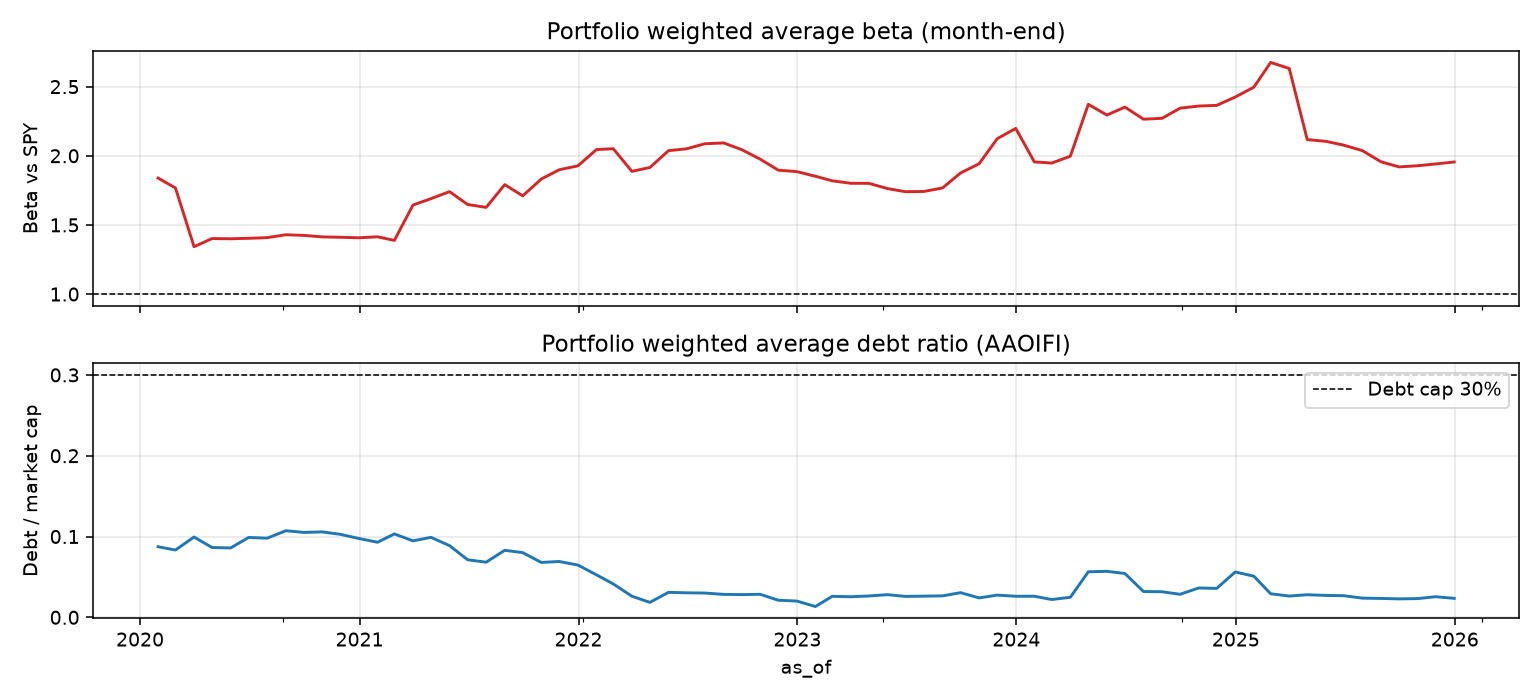
\includegraphics[width=0.88\textwidth]{figures/beta-debt-path.png}
\caption{Month-end portfolio weighted average beta versus SPY (top) and AAOIFI debt ratio (bottom). Beta stays well above 1; debt stays well below the 30\% cap.}
\label{fig:betadebt}
\end{figure}

Sharia status and beta rank are re-checked every month. A held name that fails is exited at that rebalance. It is not left in the book pending a discretionary review.

\section{Empirical performance}
\label{sec:results}

All headline numbers use the live window only: 31~January~2020 through 30~December~2025. Sharpe and Sortino use a 2\% risk-free rate. Maximum drawdown is peak-to-trough on the growth curve.

\subsection{Headline results}

\begin{table}[htbp]
\centering
\caption{Live-window performance, 31~Jan~2020 -- 30~Dec~2025.}
\label{tab:perf}
\small
\begin{tabular}{lrrrrrr}
\toprule
Book & CAGR & Vol. & Sharpe & Sortino & Max DD & Calmar \\
\midrule
High-beta low-debt tech       & 34.90\% & 43.42\% & 0.86 & 1.25 & $-48.83\%$ & 0.71 \\
Equal-weight tech sleeve      & 20.25\% & 27.91\% & 0.73 & 0.99 & $-33.54\%$ & 0.60 \\
SPY                           & 15.06\% & 20.85\% & 0.68 & 0.84 & $-33.72\%$ & 0.45 \\
S\&P~500 index                & 13.40\% & 21.04\% & 0.61 & 0.75 & $-33.92\%$ & 0.39 \\
Halal (SPUS)                  & 17.67\% & 21.77\% & 0.76 & 1.01 & $-30.80\%$ & 0.57 \\
\bottomrule
\end{tabular}
\end{table}

The high-beta book leads every benchmark on CAGR, Sharpe, Sortino, and Calmar. It also roughly doubles market volatility and takes a drawdown about 15--18~percentage points deeper than SPY or SPUS. The equal-weight sleeve beats SPY and SPUS but trails the live book by about 15~percentage points of CAGR, which is the cleanest evidence that the beta sort---not only Halal tech membership---matters in this sample.

These CAGRs are annualized figures from a sample that includes one deep growth bear (2022) and several strong upside years. They are not a forecast of 35\% a year.

\begin{figure}[htbp]
\centering

\includegraphics[width=0.88\textwidth]{figures/equity-curves.png}
\caption{Growth of \$1 in the live window. The high-beta book ends near \$6; SPY and the S\&P~500 end near \$2.1--\$2.3; SPUS near \$2.6; the equal-weight sleeve near \$3.}
\label{fig:equity}
\end{figure}

\begin{figure}[htbp]
\centering

\includegraphics[width=0.88\textwidth]{figures/rolling-excess.png}
\caption{Rolling 12-month excess return versus SPY. Excess is large in upside years and turns negative around the 2022 growth sell-off.}
\label{fig:excess}
\end{figure}

\subsection{Upside participation versus downside capture}

Table~\ref{tab:capture} is the white-paper focus metric. Upside (downside) capture is the ratio of average strategy daily return to average market daily return on days when the market is up (down).

\begin{table}[htbp]
\centering
\caption{Upside and downside capture of the high-beta book versus each market series.}
\label{tab:capture}
\begin{tabular}{lrrr}
\toprule
Benchmark & Upside capture & Downside capture & Capture spread \\
\midrule
SPY            & 1.90 & 1.80 & $+0.09$ \\
S\&P~500 index & 1.90 & 1.78 & $+0.11$ \\
SPUS           & 1.74 & 1.67 & $+0.07$ \\
\bottomrule
\end{tabular}
\end{table}

Participation is high on both sides. Versus SPY the book captures about 190\% of up-day moves and 180\% of down-day moves. The spread is only slightly positive. In plain terms: this is acceleration with a mild asymmetry, not a free lunch where upside is amplified and downside is muted. The AAOIFI debt screen removes issuer leverage, but it does not remove equity-market beta. High-beta names without corporate debt still fall hard when growth multiples compress.

\subsection{Calendar years}

\begin{table}[htbp]
\centering
\caption{Calendar-year total returns inside the live window. 2020 begins on the first invested date (31~Jan).}
\label{tab:calendar}
\begin{tabular}{lrrrr}
\toprule
Year & High-beta & SPY & S\&P~500 & SPUS \\
\midrule
2020 & 69.3\% & 16.2\% & 14.4\% & 21.7\% \\
2021 & 45.3\% & 28.7\% & 26.9\% & 35.6\% \\
2022 & $-41.3\%$ & $-18.2\%$ & $-19.4\%$ & $-22.8\%$ \\
2023 & 100.7\% & 26.2\% & 24.2\% & 34.2\% \\
2024 & 41.7\% & 24.9\% & 23.3\% & 26.5\% \\
2025 & 42.4\% & 18.6\% & 17.3\% & 20.7\% \\
\bottomrule
\end{tabular}
\end{table}

\begin{figure}[htbp]
\centering

\includegraphics[width=0.88\textwidth]{figures/calendar-year-returns.png}
\caption{Calendar-year returns. The high-beta book leads in upside years and loses roughly twice as much as the market in 2022.}
\label{fig:calendar}
\end{figure}

The shape matches the capture ratios. In 2020, 2021, 2023, 2024, and 2025 the book multiplies market upside. In 2022 it loses about $-41\%$, roughly double SPY's $-18\%$. That is the downside-capture bill for the acceleration thesis.

\subsection{Drawdowns}

\begin{figure}[htbp]
\centering

\includegraphics[width=0.88\textwidth]{figures/drawdowns.png}
\caption{Drawdowns in the live window. The high-beta trough near $-49\%$ in 2022 is deeper and longer than SPY, the S\&P~500, or SPUS.}
\label{fig:dd}
\end{figure}

Unlike the companion dual-momentum paper in this series, there is no SMA cash rule here. The book stays invested through the 2022 growth bear and marks the full drawdown. Maximum drawdown of $-48.8\%$ is the clearest single number against treating 34.9\% CAGR as a comfortable growth product.

\subsection{Does higher beta actually pay inside the sleeve?}

Cap-weight five buckets by trailing beta inside the Halal tech / clean-energy universe each month. Q5 is highest beta; Q1 is lowest.

\begin{table}[htbp]
\centering
\caption{Cap-weighted beta quintiles inside the Halal tech / clean-energy sleeve, live window.}
\label{tab:quintiles}
\small
\begin{tabular}{lrrrrrr}
\toprule
Bucket & CAGR & Vol. & Sharpe & Sortino & Max DD & Calmar \\
\midrule
Q1 (low beta)  & 11.95\% & 21.88\% & 0.53 & 0.66 & $-35.53\%$ & 0.34 \\
Q2             & 11.42\% & 27.03\% & 0.46 & 0.66 & $-39.28\%$ & 0.29 \\
Q3             & 24.91\% & 28.31\% & 0.86 & 1.17 & $-35.86\%$ & 0.69 \\
Q4             & 8.80\%  & 32.68\% & 0.36 & 0.49 & $-51.91\%$ & 0.17 \\
Q5 (high beta) & 35.73\% & 43.27\% & 0.88 & 1.27 & $-48.83\%$ & 0.73 \\
\bottomrule
\end{tabular}
\end{table}

\begin{figure}[htbp]
\centering

\includegraphics[width=0.88\textwidth]{figures/quintile-growth.png}
\caption{Growth of \$1 by beta quintile. Q5 leads; the middle of the distribution is not ordered.}
\label{fig:qgrowth}
\end{figure}

\begin{figure}[htbp]
\centering

\includegraphics[width=0.88\textwidth]{figures/quintile-spread.png}
\caption{Cumulative Q5 minus Q1 relative wealth. The spread ends strongly positive after a near-wipeout through the 2022 relative drawdown.}
\label{fig:qspread}
\end{figure}

Q5 dominates on CAGR and matches the live book's risk profile. The ladder is not monotonic: Q3 is a strong second, while Q4 is the worst bucket. The live rule of ``own the top quintile'' is therefore supported as a selection device, not as evidence of a smooth beta premium across the sleeve.

\section{Attribution}
\label{sec:attrib}

Section~\ref{sec:results} shows that the book won on compound growth and risk-adjusted ratios while paying for that win in drawdown depth. This section asks what that win looks like structurally.

\subsection{Equal-weight twin versus beta tilt}

The equal-weight Halal tech / clean-energy sleeve holds the same screened universe without ranking on beta. It returns 20.3\% CAGR with a $-33.5\%$ drawdown---better than SPY and SPUS, worse than the live book. The gap of about 15~percentage points of CAGR is the contribution of the top-quintile beta sort in this sample, on top of already being in Halal tech and clean energy. That twin is the cleanest attribution control available in the notebook: same screens, same sleeve, different only in whether high-beta names are overweighted.

\subsection{Portfolio beta and debt}

Figure~\ref{fig:betadebt} shows that the live book runs a market beta of roughly 1.7--2.2 for most of the sample, peaking near 2.6 in 2025, while weighted AAOIFI debt stays mostly below 5\% and always below the 30\% cap. The strategy therefore does what the title promises mechanically: high equity beta, low corporate debt. ``Without leverage risk'' here means without \emph{issuer} leverage and without \emph{portfolio} margin. It does not mean low equity risk.

\subsection{Concentration and sector identity}

By construction the book is a technology and clean-energy sleeve. Cap-weighting inside the top beta quintile further concentrates capital into the largest accelerators. At the final rebalance Nvidia alone was 46.6\% of the portfolio. Any claim that the result is ``pure beta'' rather than ``Nvidia and friends in a Halal tech boom'' would require a position-capped or sector-neutral twin that this paper does not run.

\subsection{What can and cannot be isolated}

The equal-weight twin isolates the beta tilt from sleeve membership. Capture ratios isolate the upside/downside asymmetry that motivated the study. What remains unidentified is how much of Q5's edge is beta itself versus a handful of mega-cap winners that happened to sit in Q5 during 2023--2025. Without a name-capped twin and without a longer sample that includes a high-rate recession beyond 2022, I cannot separate those stories cleanly.

\section{Limitations and implementation friction}
\label{sec:limits}

\subsection{Turnover, slippage, and net CAGR}

Turnover is one-way: half the $\ell_1$ weight change between consecutive month-end books. Trading-cost drag assumes 10~basis points per one-way turn.

\begin{table}[htbp]
\centering
\caption{Implementation friction on the live high-beta book.}
\label{tab:friction}
\begin{tabular}{lr}
\toprule
Item & Value \\
\midrule
Rebalances with holdings           & 72 \\
Median names held                  & 16 \\
Average one-way turnover / month   & 18.4\% \\
Median one-way turnover / month    & 7.3\% \\
Implied annualized one-way turnover & $\approx$ 221\% \\
Assumed cost per one-way trade     & 10~bp \\
CAGR gross of trading costs        & 34.90\% \\
CAGR net of trading costs          & 34.60\% \\
\bottomrule
\end{tabular}
\end{table}

\begin{figure}[htbp]
\centering

\includegraphics[width=0.88\textwidth]{figures/turnover.png}
\caption{One-way turnover at each month-end rebalance. Most months are quiet; a minority of rebalances reshuffle half or more of the book.}
\label{fig:turnover}
\end{figure}

Average monthly turnover of 18.4\% annualizes to roughly 220\% one-way. At 10~bp the estimated drag is only about 30~bp of CAGR in this sample (34.90\% gross to 34.60\% net), because many months churn little while a few months rotate hard. Real slippage on mid-cap clean-energy names and on forced exits after compliance fails could be wider. I do not model market impact, borrow, or taxes.

\subsection{Purification drag}

Impure income that may require purification is reported, not ignored, in the companion papers in this series. This notebook does not recompute a full dividend-purification panel for every holding day; several tech names in the sleeve have low or zero ordinary dividends, which tends to keep purification drag small relative to a 35\% CAGR. Missing interest-income tags remain a gap, not evidence of zero drag.

\subsection{Point-in-time compliance}

Screens are applied at each rebalance. Failed names are sold then. There is no intra-month compliance monitor. Sector exclusions use the current S\&P list and current activity labels, not the 2020 membership file. That is survivorship and look-ahead in the universe construction, even though the filings themselves use point-in-time dates where available.

\subsection{Data and construction issues}

SEC companyfacts supply the long fundamental history used for AAOIFI ratios. Yahoo statements are the fallback when no CIK exists. Restatements and XBRL tag mapping are not audited here. Prices come from yfinance adjusted closes. Cap-weighting two share classes of the same issuer, where both appear, would inflate that issuer relative to a single-listing index; that construction risk exists for any S\&P-based sleeve.

There is no position cap, so Nvidia-scale winners can dominate. The top-quintile cutoff and the 252-day beta window were fixed before the full run. They were not optimized on a hold-out, but any design choice inside a six-year growth-friendly window is still partly in-sample.

\subsection{What this paper does not show}

There is no 2008, no rising-rate recession beyond 2022, no hold-out after a rule freeze, and no name-capped twin. Capture spreads are only mildly positive. Downside capture near $1.8\times$ means the strategy is not ``growth without left-tail risk.'' Beating SPY and SPUS with an unconstrained high-beta tech book in 2020--2025 is interesting. It is not evidence that the same rule survives every cycle, which was the original participation-versus-capture question.

\section{Conclusion}
\label{sec:conc}

A cap-weighted book of AAOIFI-screened technology and clean-energy names selected by top-quintile trailing beta versus SPY returned 34.9\% compound annual growth from early 2020 through 2025, against 15.1\% for SPY and 17.7\% for SPUS. The equal-weight sleeve at 20.3\% CAGR shows that the beta sort added material return on top of Halal tech membership. Portfolio debt stayed low; portfolio equity beta did not. Upside capture near $1.9\times$ came with downside capture near $1.8\times$ and a maximum drawdown of $-48.8\%$.

The product shape is coherent enough to keep studying: low-debt screens, a tech/clean-energy sleeve, high-beta selection, and long-only cap-weighting. It is not ready to promote to a live mandate. A second paper would need a frozen rule, point-in-time index membership, a hard name cap (for example 5--8\%), explicit purification accounting, and at least one more independent down year. If a capped twin still beats SPUS on Calmar after costs with a clearly favorable capture spread, the acceleration claim has more to stand on. If it does not, the 34.9\% CAGR in this sample is mostly concentrated mega-cap beta in a friendly window.

\paragraph{Reproduction.}
Run \texttt{code.ipynb} in this paper's folder with \texttt{FAST\_MODE=False} and dates 2020-01-01 to 2025-12-31. Figures are stored alongside the notebook. The public repository is \url{https://github.com/regional-specter/Monterey-Finance}.

\bibliographystyle{plainnat}
\begin{thebibliography}{9}

\bibitem[AAOIFI(2020)]{aaoifi21}
Accounting and Auditing Organization for Islamic Financial Institutions, 2020.
\newblock Financial Paper (Shares and Bonds).
\newblock Shari'ah Standard No.~21, AAOIFI, Manama.

\bibitem[Black(1972)]{black1972}
Black, F., 1972.
\newblock Capital market equilibrium with restricted borrowing.
\newblock Journal of Business 45, 444--455.

\bibitem[Derigs and Marzban(2008)]{derigs2008}
Derigs, U., Marzban, S., 2008.
\newblock Review and analysis of current Shariah-compliant equity screening practices.
\newblock International Journal of Islamic and Middle Eastern Finance and Management 1, 285--303.

\bibitem[Fama and French(1992)]{fama1992}
Fama, E.~F., French, K.~R., 1992.
\newblock The cross-section of expected stock returns.
\newblock Journal of Finance 47, 427--465.

\end{thebibliography}

\end{document}
